\documentclass[margin=0mm,tikz]{standalone}

\usepackage{tikz}
\usepackage{xcolor}
\usepackage{ifthen}
\usepackage{amsmath}

\usetikzlibrary{positioning}
\usetikzlibrary{fit}
\usetikzlibrary{calc}
\usetikzlibrary{arrows.meta}
\usetikzlibrary{quotes}

\pgfdeclarelayer{background}
\pgfsetlayers{background,main}

% -----------------------
% colors
% -----------------------
\definecolor{forwardcolor}{RGB}{150, 150, 150}
\definecolor{operatorcolor}{RGB}{136, 150, 186}
\definecolor{convcolor}{RGB}{175, 0, 23}
\definecolor{skipcolor}{RGB}{218, 138, 0}
\definecolor{reccolor}{RGB}{113, 0, 162}
\definecolor{catcolor}{RGB}{255, 0, 0}

% Set background color
%\pagecolor{white}

% -----------------------
% colors
% -----------------------

\tikzstyle{operator} = [
    circle,
    draw,
    top color = gray!20!white,
    bottom color = gray!30!white, 
    text=black,
    minimum size=0.5cm,
    inner sep=0pt
]

\tikzstyle{projection} = [
	midway,
	draw,
	rounded corners=1pt,
	%top color = black!70!white,
	%bottom color = black!80!white, 
	fill=white!60!black,,
	text=white,
	minimum size=0.5cm,
	inner sep=2pt,
	rotate=0,
]

\tikzstyle{forward} = [-{Latex[length=2pt, width=6pt]}, line width=2pt, forwardcolor]
\tikzstyle{skip} = [-{Latex[length=3pt, width=5pt]}, line width=2pt, skipcolor]

\tikzset{
	annotated cuboid/.pic={
		\tikzset{%
			every edge quotes/.append style={midway, auto},
			/cuboid/.cd,
			#1
		}
		
		% coordinate scheme of the cube
		%
		%    e---------h
		%   /|        /|
		%  / |       / |
		% a---------d  |
		% |  |      |  |
		% |  f------|--g
		% | /       | /
		% |/        |/
		% b---------c
		
		% Set up the corner coordinates of the cube
		\coordinate (a) at (-\cwidth*\cscale*0.5, \cheight*\cscale*0.5, 0);
		\coordinate (b) at (-\cwidth*\cscale*0.5, -\cheight*\cscale*0.5, 0);
		\coordinate (c) at (\cwidth*\cscale*0.5, -\cheight*\cscale*0.5, 0);
		\coordinate (d) at (\cwidth*\cscale*0.5, \cheight*\cscale*0.5, 0);
		\coordinate (e) at (-\cwidth*\cscale*0.5, \cheight*\cscale*0.5, -\cdepth*\cscale);
		\coordinate (f) at (-\cwidth*\cscale*0.5, -\cheight*\cscale*0.5, -\cdepth*\cscale);
		\coordinate (g) at (\cwidth*\cscale*0.5, -\cheight*\cscale*0.5, -\cdepth*\cscale);
		\coordinate (h) at (\cwidth*\cscale*0.5, \cheight*\cscale*0.5, -\cdepth*\cscale);
		
		
		% Clip the cube image to the outer coordinates
		\clip (a) -- (b) -- (c) -- (g) -- (h) -- (e) -- cycle;
		
		%
		% Draw the cube
		
		\draw[\ccolor, dashed, very thick] (f) -- (g);
		\ifthenelse{\cat=0}{
			\draw[\ccolor, dashed, very thick] (f) -- (b);
			\draw[\ccolor, dashed, very thick] (f) -- (e);
		}{
			\draw[catcolor, dashed, very thick] (f) -- (b);
			\draw[catcolor, dashed, very thick] (f) -- (e);
		}
		% Dashed, hidden lines
		%\draw[\ccolor, dashed, very thick] (f) -- (b);
		%\draw[\ccolor, dashed, very thick] (f) -- (g);
		%\draw[\ccolor, dashed, very thick] (f) -- (e);
		
		% Faces
		\draw[fill=\ccolor, opacity=0.6] (a) -- (b) -- (c) -- (d) -- cycle;  % front
		\draw[fill=\ccolor, opacity=0.6] (a) -- (d) -- (h) -- (e) -- cycle;  % top
		\draw[fill=\ccolor, opacity=0.6] (d) -- (c) -- (g) -- (h) -- cycle;  % right
		
		% Redraw edges of the faces
		\draw[\ccolor, very thick] (a) -- (b) -- (c) -- (d) -- cycle;  % front
		\draw[\ccolor, very thick] (a) -- (d) -- (h) -- (e) -- cycle;  % top
		\draw[\ccolor, very thick] (d) -- (c) -- (g) -- (h) -- cycle;  % right
		
		\ifthenelse{\cat=1}{
			\draw[catcolor, dashed, very thick] (b) -- (a) -- (e);
		}{}
		
		% Draw annotations
		\draw [\ccolor] (a) edge ["\color{black}\textbf{\rotatebox{0}{\lheight}}"] (b);
		\draw [\ccolor] (b) edge ["\color{black}\textbf{\lwidth}"] (c);
		
		% Define the node for this kernel
		\node [anchor=north west, minimum width=\cwidth*\cscale cm, minimum height=\cheight*\cscale cm] (\clabel) at (a) {};
		
	},
	/cuboid/.search also={/tikz},
	/cuboid/.cd,
	width/.store in=\cwidth,
	height/.store in=\cheight,
	depth/.store in=\cdepth,
	units/.store in=\cunits,
	scale/.store in=\cscale,
	label/.store in=\clabel,
	lwidth/.store in=\lwidth,
	lheight/.store in=\lheight,
	ccolor/.store in=\ccolor,
	cat/.store in=\cat,
	width=1,
	height=1,
	depth=1,
	units=cm,
	scale=1.0,
	label=dummy,
	lwidth=2,
	lheight=2,
	ccolor=white!70!black,
	cat=0,
}

\begin{document}
	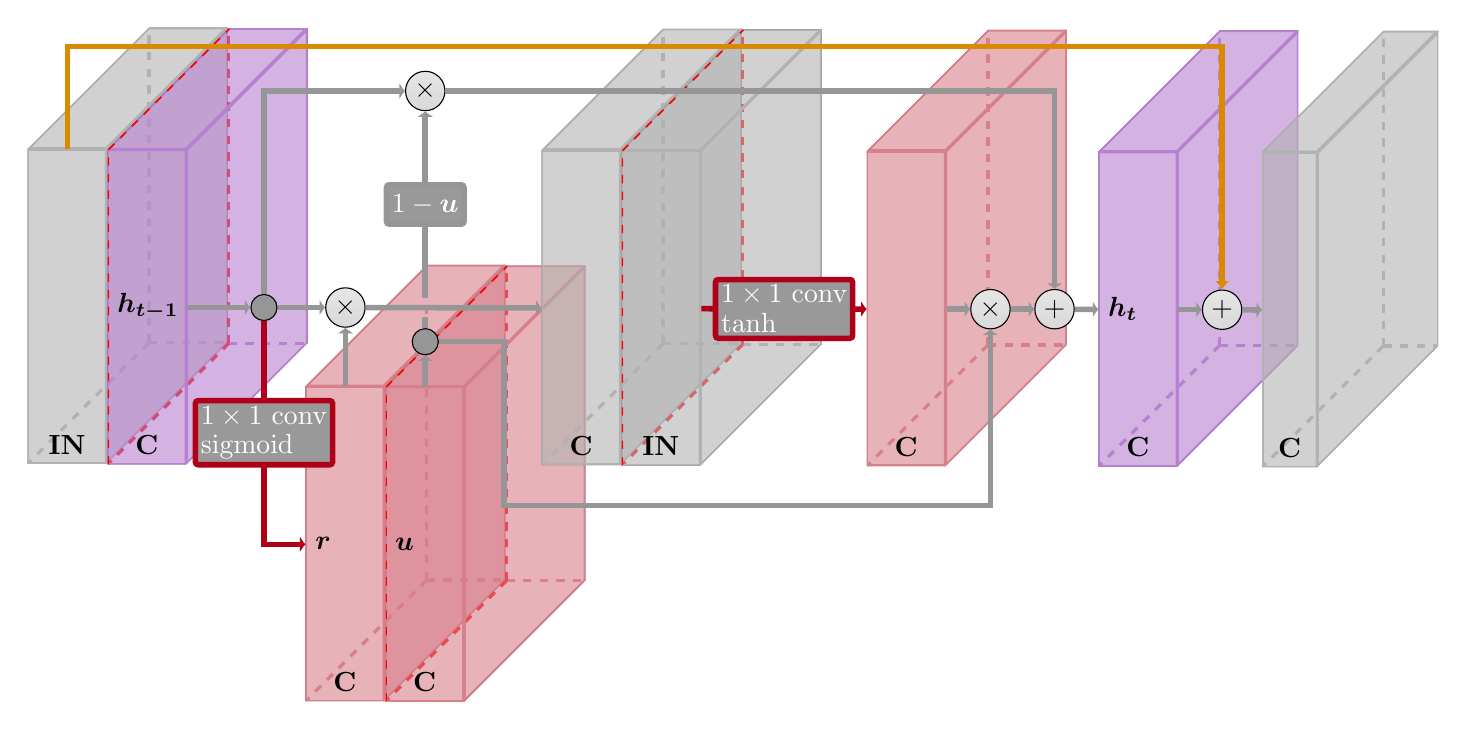
\begin{tikzpicture}
	
	% Maps
	
	% Input [ x | h_t-1 ]
	\pic {annotated cuboid={width=1.0, height=4, depth=4, units=, label=input, lwidth=IN, lheight=}};
	\pic [right=0.5cm of input] {annotated cuboid={width=1.0, height=4, depth=4, units=, label=h_t_1, lwidth=C, lheight=$\boldsymbol{h_{t-1}}$, ccolor=white!50!reccolor, cat=1}};

	\node [right=0.8 of h_t_1, draw=black, circle, fill=forwardcolor] (hhelper) {};
	
	% Reset and update gates [ r | u ]
	\pic [right=2.0cm of h_t_1, yshift=-3cm] {annotated cuboid={width=1.0, height=4, depth=4, units=, label=reset, lwidth=C, lheight=$\boldsymbol{r}$, ccolor=white!50!convcolor}};
	\pic [right=0.5cm of reset] {annotated cuboid={width=1.0, height=4, depth=4, units=, label=update, lwidth=C, lheight=$\boldsymbol{u}$, ccolor=white!50!convcolor, cat=1}};
	
	\node [operator] at (hhelper -| reset) (mul1) {$\times$};	
	\node [above=3.5cm of update, operator] (mul2) {$\times$};
	\node at (update |- hhelper) (udummy) {};
	\node [above=0.4cm of update, draw=black, circle, fill=forwardcolor] (uhelper) {};
	
	% Intermediate z [ r*h_t_1 | x ]	
	\pic [right=5.0cm of h_t_1] {annotated cuboid={width=1.0, height=4, depth=4, units=, label=zl, lwidth=C, lheight=}};
	\pic [right=0.5cm of zl] {annotated cuboid={width=1.0, height=4, depth=4, units=, label=zr, lwidth=IN, lheight=, cat=1}};
	\pic [right=2.6cm of zr] {annotated cuboid={width=1.0, height=4, depth=4, units=, label=z, lwidth=C, lheight=, ccolor=white!50!convcolor}};
	
	% Mul3, Add1, and new hidden state
	\node[operator, right=0.3cm of z] (mul3) {$\times$};
	\node[operator, right=0.3cm of mul3] (add1) {$+$};
	\pic [right=0.8cm of add1] {annotated cuboid={width=1.0, height=4, depth=4, units=, label=h_t, lwidth=C, lheight=$\boldsymbol{h_t}$, ccolor=white!50!reccolor}};
	
	% Residual and output
	\node[operator, right=0.3cm of h_t] (add2) {$+$};
	\pic [right=0.6cm of add2] {annotated cuboid={width=0.7, height=4, depth=4, units=, label=output, lwidth=C, lheight=}};

	
	% Arrows
	\draw[forward] (h_t_1) -- (hhelper);
	\draw[forward, convcolor] (hhelper) -- (hhelper |- reset)  node[projection] {\shortstack[l]{$1\times1$ conv\\sigmoid}} -- (reset);
	\draw[forward] (hhelper) -- (hhelper.north |- mul2) -- (mul2);
	
	\draw[forward] (hhelper) -- (mul1);
	\draw[forward] (reset) -- (mul1);
	\draw[forward] (mul1) -- (zl);
	\draw[forward] (update) -- (uhelper);
	\draw[forward] (uhelper) -- (udummy) -- (mul2)  node[projection] {\shortstack[l]{$1-\boldsymbol{u}$}};
	\draw[forward] (uhelper) --++ (1, 0) -- ([xshift=1.0cm, yshift=0.5cm]uhelper |- update) -- ([yshift=0.5cm]update -| mul3) -- (mul3);
	\draw[forward] (mul2) -- (mul2 -| add1) -- (add1);
	
	\draw[forward, convcolor] (zr) -- (z)  node[projection] {\shortstack[l]{$1\times1$ conv\\tanh}};
	\draw[forward] (z) -- (mul3);
	\draw[forward] (mul3) -- (add1);
	\draw[forward] (add1) -- (h_t);
	\draw[forward] (h_t) -- (add2);
	\draw[forward] (add2) -- (output);
	
	
	
	
	%\draw[forward, convcolor] (c1) -- (c2) node[projection] {\shortstack[l]{$3\times3$ conv\\GELU}};
	%\draw[forward, convcolor] (c2) -- (c3) node[projection] {\shortstack[l]{$1\times1$ conv}};
	%\draw[forward] (zr) -- (plus);
	\draw[skip] (input.north) --++ (0, 1.3cm) -- ([yshift=1.3cm]input.north -| add2) -- (add2.north);
	%\draw[forward] (plus) -- (output) node[projection] {ReLU};
	%\draw[forward] (plus) -- (output);
		
	\end{tikzpicture}
\end{document}